\documentclass[aspectratio=169,10pt]{beamer}
\usepackage{fontspec}
\usepackage{assets/ide-beamer}
\hypersetup{colorlinks=true,urlcolor=IDERed}

\title{Artificial Intelligence in the Knowledge Economy}
\author{John Barraza}
\institute{Universidad del Pacífico · AI Economic Modelling}
\date{September 2026}

\begin{document}

% 1
\begin{frame}[plain]
  \vspace{.45cm}
  {\color{IDERed}\large\bfseries REPOSITORY 05}\par\vspace{.28cm}
  {\usebeamerfont{title}\color{IDENavy}Artificial Intelligence in the\\Knowledge Economy}\par\vspace{.28cm}
  {\large Ide \& Talamàs (2025), \textit{Journal of Political Economy}}\par\vspace{.52cm}
  \begin{tikzpicture}
    \draw[IDENavy,line width=2pt] (0,0)--(11.5,0);
    \draw[IDERed,line width=5pt] (8.2,0)--(11.5,0);
  \end{tikzpicture}
  \vfill
  {\small John Barraza · Universidad del Pacífico}\hfill{\small\href{\repoURL}{github.com/johnbarraza/ai-05-ide}}
\end{frame}

% 2
\begin{frame}{1. The paper and the agent's problem}
\small
\begin{columns}[T,onlytextwidth]
  \column{.43\textwidth}
  \tagpill{Question}\par\vspace{.18cm}
  How do AI capability and autonomy reorganize knowledge work, output, and wages?
  \vspace{.28cm}
  \begin{block}{One mechanism}
  Workers attempt problems; solvers handle exceptions. AI changes matching, span of control, and surplus shares.
  \end{block}
  \vspace{.12cm}
  \bluepill{Technology}\quad $n(z)=\dfrac{1}{h(1-z)}$

  \column{.53\textwidth}
  \tagpill{Competitive firm's choice}\par\vspace{.12cm}
  For human worker $z$, choose solver $s\ge z$:
  \[
    \max_{s\ge z}\ \Pi^{nA}_2(s,z)
    =n(z)[s-w(z)]-w(s).
  \]
  Autonomous AI adds the alternatives
  \[
  \Pi_1^A=z_{AI}-r,\qquad
  \Pi_2^{tA}=n(z)\,[z_{AI}-w(z)]-r,
  \]
  \[
  \Pi_2^{bA}=n(z_{AI})\,[s-r]-w(s).
  \]
  Free entry: the chosen structure earns zero profit.
\end{columns}
\paperref{Accepted manuscript, Sections 3.1--3.2, equations (1)--(4).}
\end{frame}

% 3
\begin{frame}{2. Main result: capability and autonomy are distinct}
\scriptsize
\textbf{Maintained environment:} $z\in[0,1]$ observable; $g$ continuous and strictly positive; $x\sim U[0,1]$; $h<h_0$; at most two layers; identical compute abundant relative to human time; $z_{AI}\in[0,1)$.
\vspace{.12cm}

\begin{columns}[T,onlytextwidth]
\column{.49\textwidth}
\begin{block}{Proposition 5 · autonomous AI}
Let $B=\{z\le z_{AI}:w^*(z)>w(z)\}$ and $T=\{z\ge z_{AI}:w^*(z)>w(z)\}$. Then
\[
B\ne\varnothing\iff z_{AI}>\bar z_{AI},
\quad \bar z_{AI}\in\operatorname{int}W,
\]
\[
T\ne\varnothing\quad\forall z_{AI}\in[0,1).
\]
The top claim can fail for $h\ge h_0$ and does not include $z_{AI}=1$.
\end{block}

\column{.49\textwidth}
\begin{alertblock}{Proposition 6 · non-autonomous AI}
Unique efficient equilibrium, $r^\star=0$. If $z_{AI}\le w(0)$, AI is unused. If $z_{AI}>w(0)$, only the bottom uses it as solver. In either case:
\begin{enumerate}\scriptsize
  \item $Y^*>Y^\star$;
  \item some $z>0$ has $w^\star(z)\le w(z)$, strictly if active;
  \item near zero, $w^\star\ge\max\{w,w^*\}$, strictly if active;
  \item near one, $w^\star\le w^*$, strictly for $z\ne1$.
\end{enumerate}
\end{alertblock}
\end{columns}
\vspace{.04cm}
\textbf{Intuition:} autonomy changes feasible roles; \condition{capability sets both the bottom-winner and adoption thresholds}.
\end{frame}

% 4
\begin{frame}{3. What I did: a three-type Lean audit}
\small
\begin{columns}[T,onlytextwidth]
\column{.48\textwidth}
Let $L<M<H$, $a=z_{AI}$, and
\[
n_L=\frac{1}{h(1-z_L)}.
\]
Autonomous AI can produce alone, so $r^*=a$. Zero profit for AI solving for $L$ gives
\[
n_L(a-w_L^A)-a=0
\quad\Rightarrow\quad
\boxed{w_L^A=a[1-h(1-z_L)]}.
\]
Hence
\[
\boxed{L\text{ wins}\iff
a>\bar a_L=\frac{w_L^0}{1-h(1-z_L)}}.
\]

\column{.48\textwidth}
Non-autonomous AI leaves compute idle, so $r^\star=0$. Conditional on adoption,
\[
n_L(a-w_L^N)=0\Rightarrow w_L^N=a,
\]
and Proposition 6 requires $a>w(0)$. Therefore
\[
\boxed{w_L^N-w_L^A=ah(1-z_L)>0}.
\]
\begin{alertblock}{What the exercise isolates}
Capability turns adoption and bottom gains on; autonomy changes AI's outside option and who captures surplus.
\end{alertblock}
\end{columns}
\paperref{Discrete extension: SymPy checks plus 3 Lean-verified proof endpoints in lean/.}
\end{frame}

% 5
\begin{frame}{4. Where I did not believe the AI}
\small
\begin{columns}[T,onlytextwidth]
\column{.52\textwidth}
\IfFileExists{hand/derivation.jpg}{%
  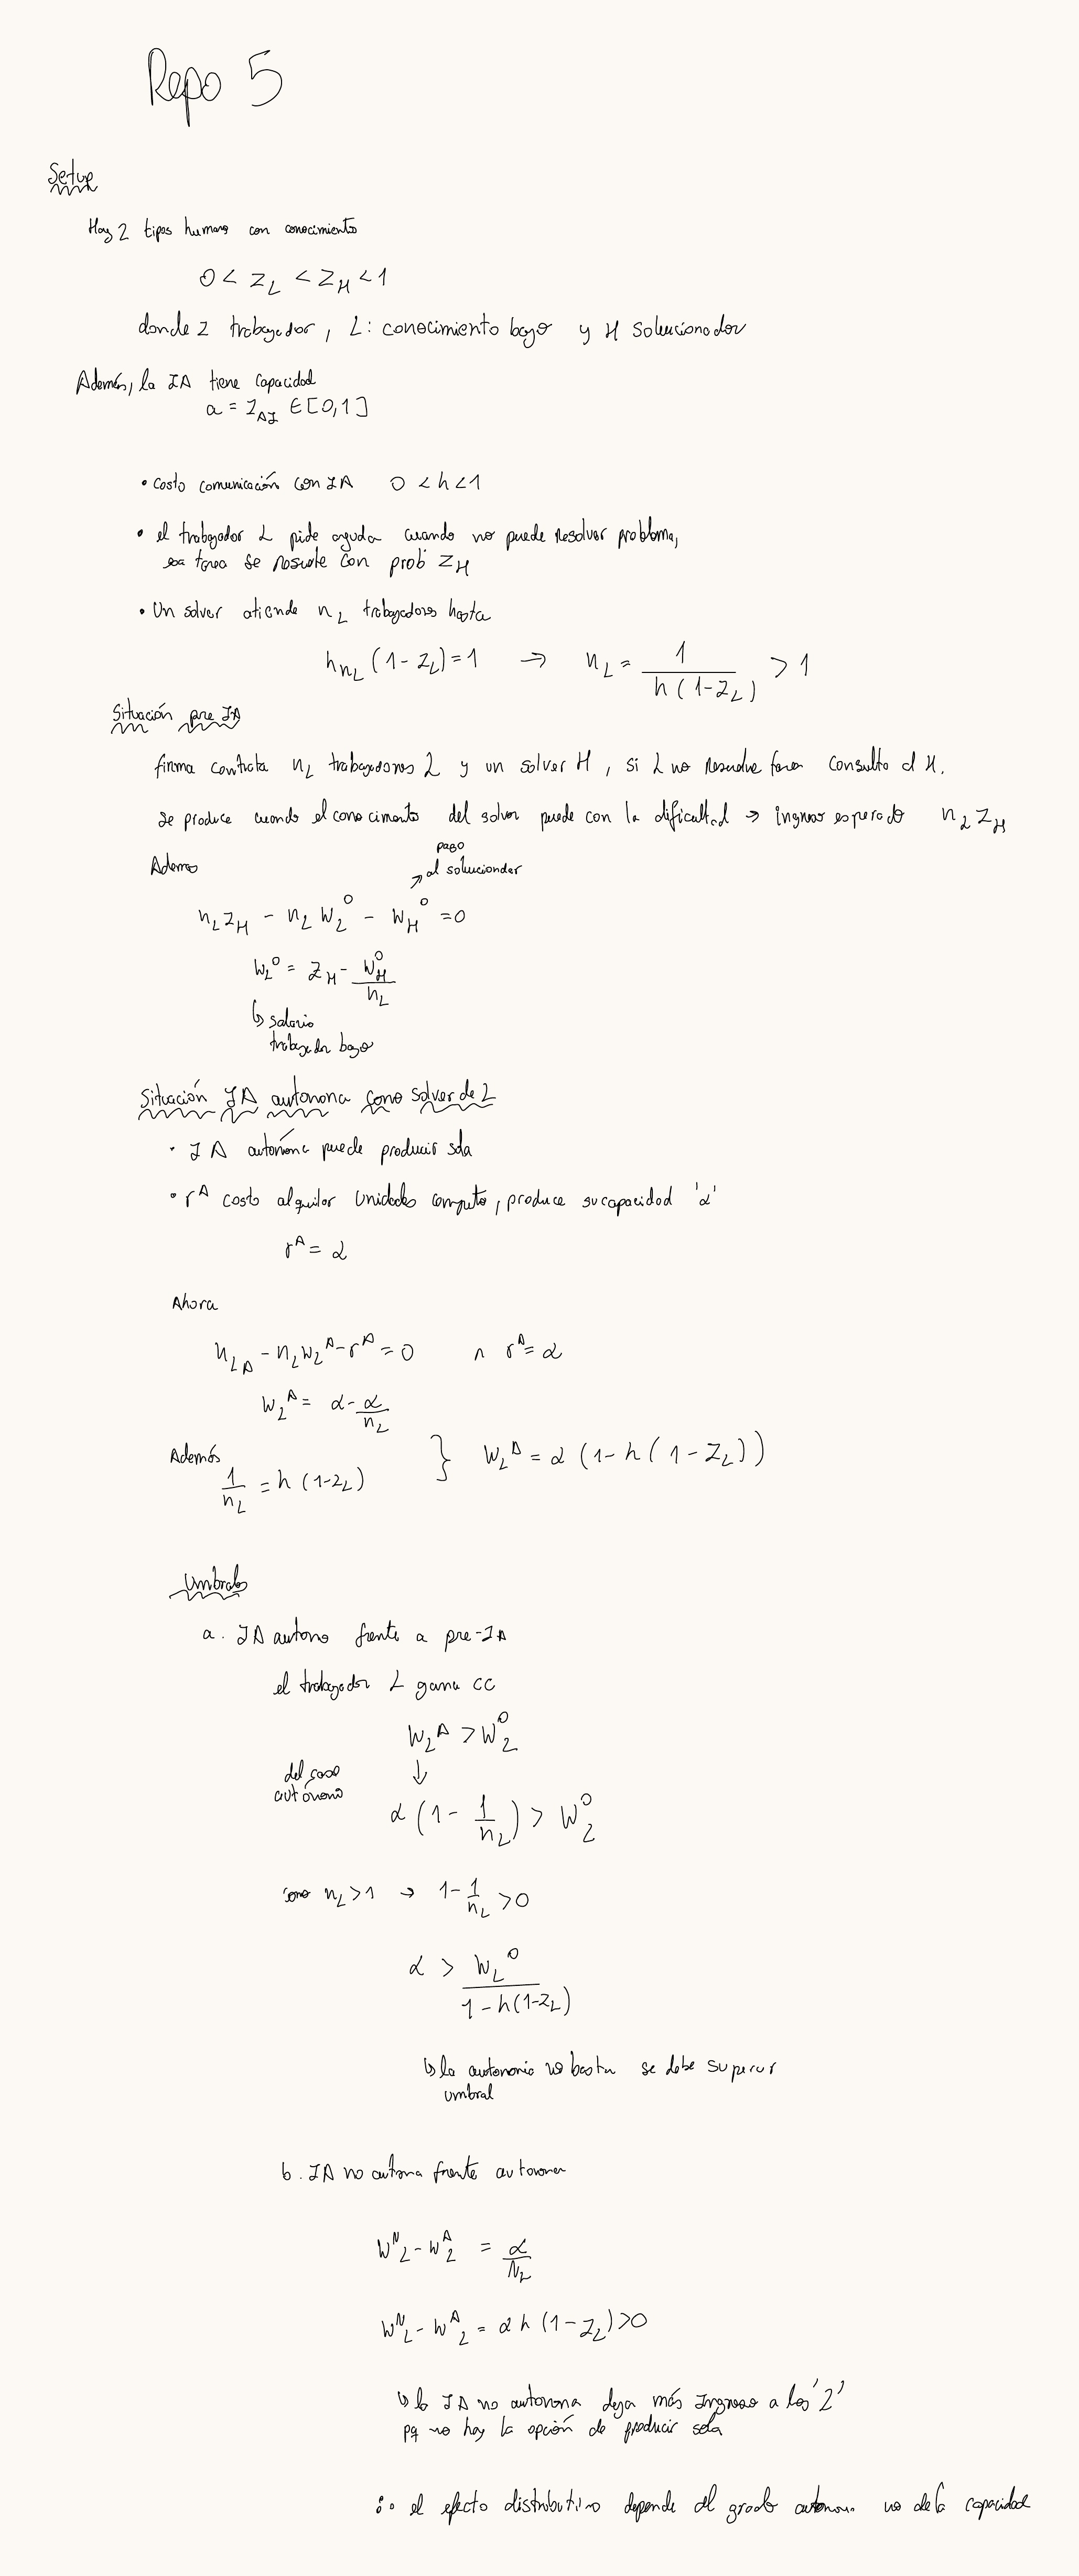
\includegraphics[width=\linewidth,height=.68\textheight,keepaspectratio]{hand/derivation.jpg}%
}{\IfFileExists{hand/derivation.png}{%
  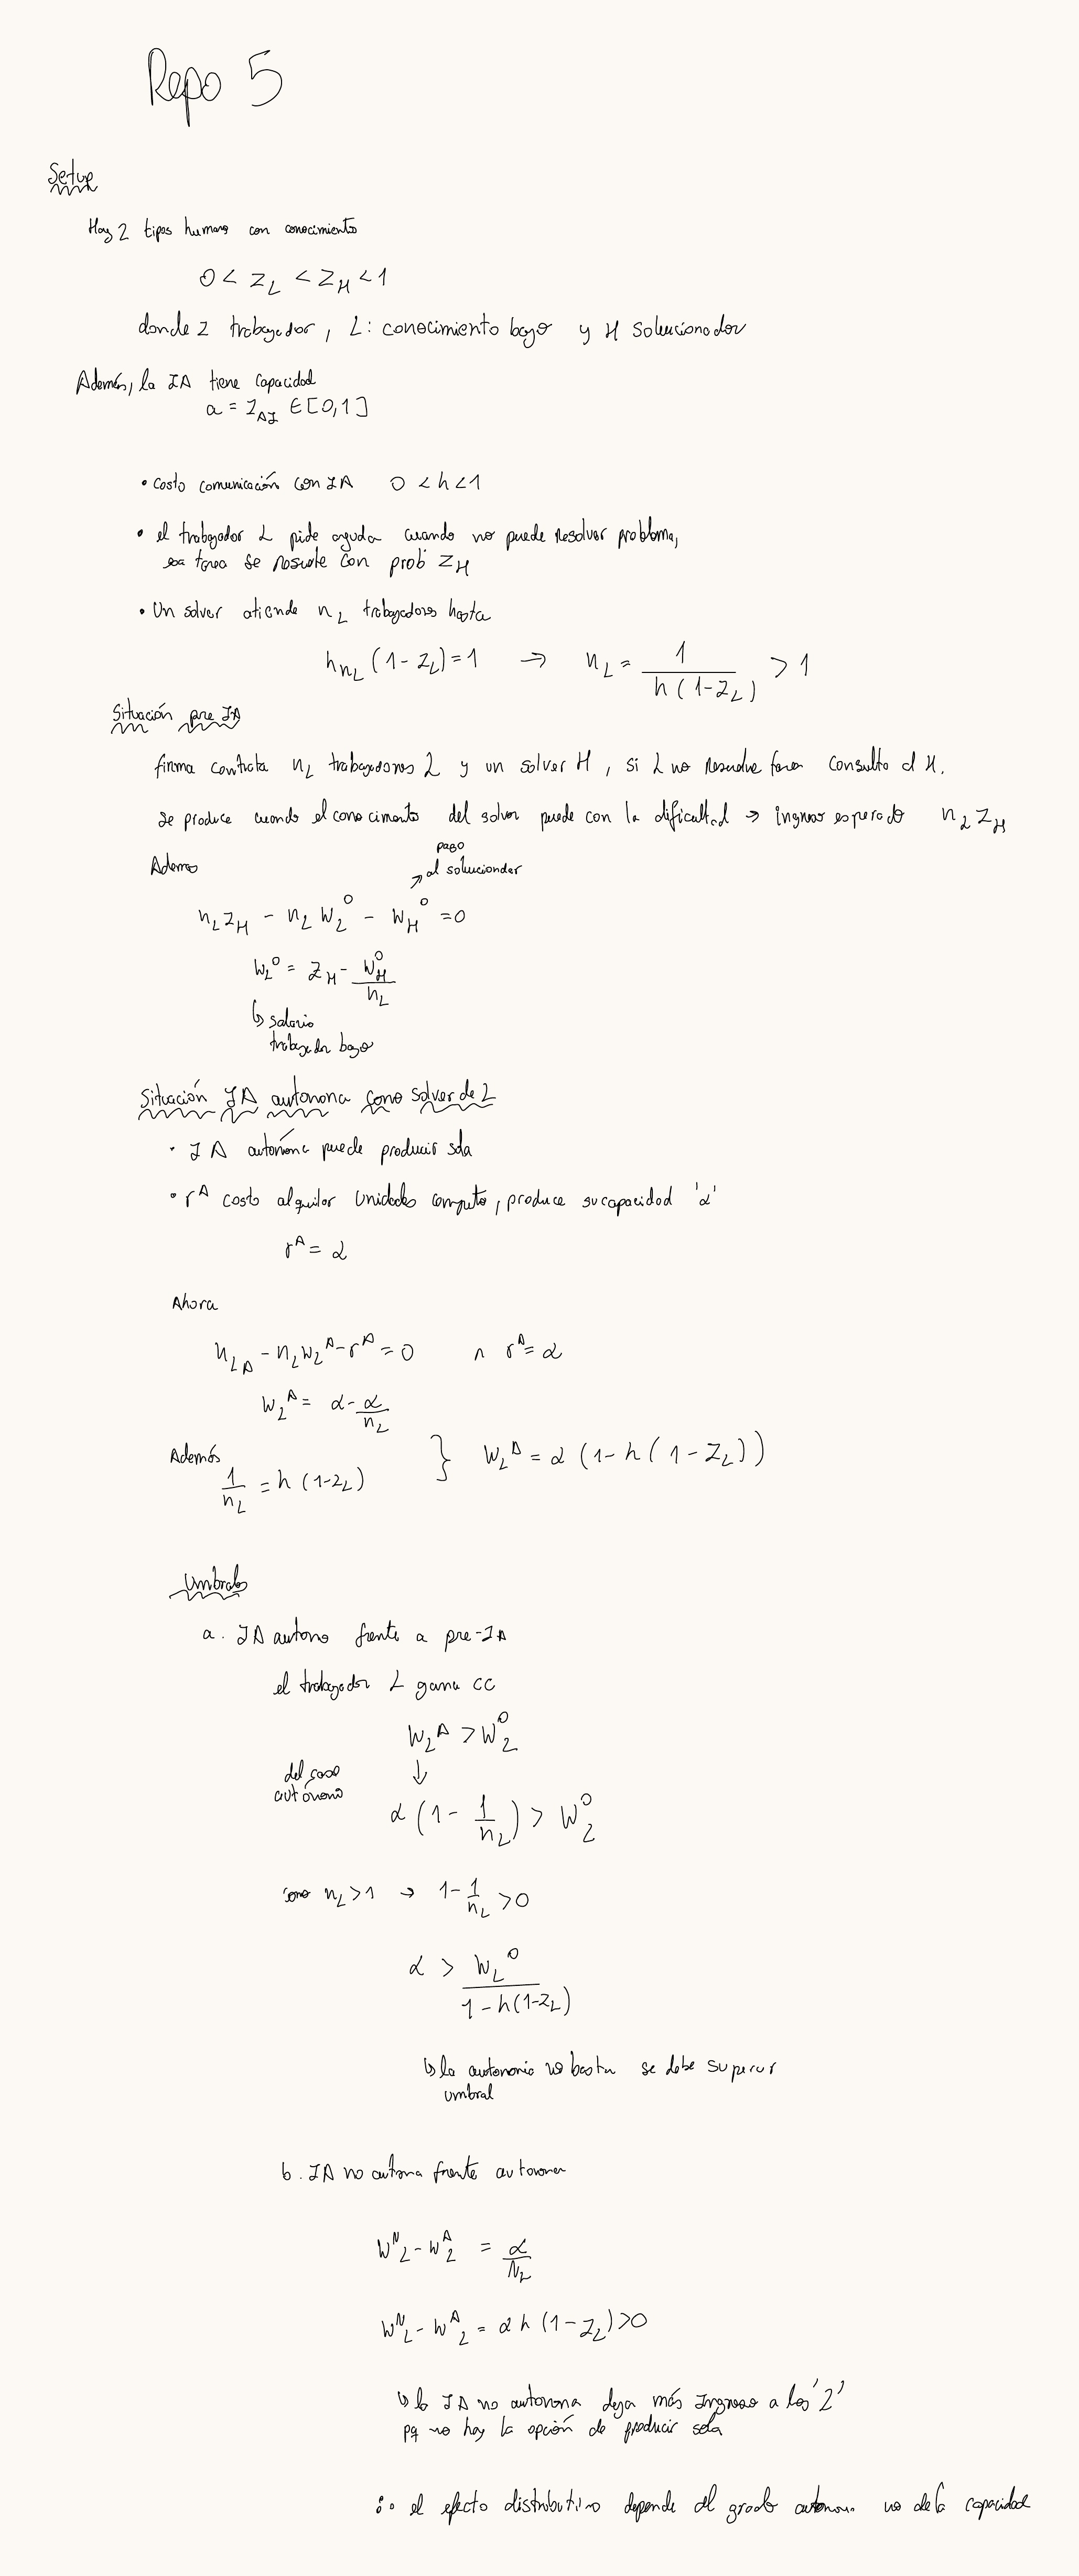
\includegraphics[width=\linewidth,height=.68\textheight,keepaspectratio]{hand/derivation.png}%
}{%
  \begin{alertblock}{Insert authentic evidence}
  Add your own photo as \texttt{hand/derivation.jpg}, then recompile. The equations to reproduce are in \texttt{hand/README.md}.
  \end{alertblock}
}}
\column{.44\textwidth}
The tempting AI answer was:
\begin{quote}
“Distributional effects are driven by autonomy, not capability.”
\end{quote}
\begin{alertblock}{My verdict: incomplete}
Prop. 5 requires $z_{AI}>\bar z_{AI}$ for autonomous bottom winners. Prop. 6 requires $z_{AI}>w(0)$ before non-autonomous AI is even used.
\end{alertblock}
Autonomy determines the role set; capability determines whether the relevant regime activates. The paper has two dimensions, not one.
\end{columns}
\paperref{Accepted manuscript, Propositions 5--6, pp. 25--28.}
\end{frame}

\end{document}
